\documentclass[11pt,twoside,slovak,a4paper]{article}

\usepackage[slovak]{babel}
\usepackage[IL2]{fontenc} % lepšia sadzba písmena Ľ než v T1
\usepackage[utf8]{inputenc}
\usepackage{graphicx}
\usepackage{url} % príkaz \url na formátovanie URL
\usepackage{hyperref} % odkazy v texte budú aktívne (pri niektorých triedach dokumentov spôsobuje posun textu)

\usepackage{cite}

\oddsidemargin=0cm % text na neparnych stranach bude vycentrovany lebo margin = 0
\evensidemargin=0cm
\textwidth=16.5cm % sirka textu na strane

\pagestyle{headings}

\title{Využitie statickej analýzy kódu pri vývoji softwaru}

\author{Lukáš Častven\\[2pt]
	{\small Slovenská technická univerzita v Bratislave}\\
	{\small Fakulta informatiky a informačných technológií}\\
	{\small \texttt{xcastven@stuba.sk}}
	}

\date{\small  5. november 2021}

\begin{document}

\maketitle

\begin{abstract}
	Statická analýza je proces, pri ktorom je počítačový kód zanalyzovaný bez samotného spúšťania kódu.
	Po tejto procedúre, sú programátorovi prezentované nájdené chyby, ich možný spôsob opravy a aj varovania
	o menej závažných nedostatkoch a ich riešenia. Pomocou tejto metódy dokážeme v celom analyzovanom projekte
	zlepšiť kvalitu kódu a udržať konzistentný štýl, ktorý taktiež spĺňa osvedčené postupy pri vývoji softvéru.
	Veľkou výhodou je tiež urýchlenie hľadania chýb a softvérových defektov v porovnaní s manuálnou kontrolou.
	V tomto článku pochopíme, prečo developeri používajú nástroje statickej analýzy, ako ich používajú
	na opravu a zlepšenie kódu a ako ich implementujú do ich pracovného prostredia.~\cite{Main}
\end{abstract}

\pagebreak

\section{Úvod}

\section{Princípy statickej analýzy}
\subsection{Čo je statická analýza}
\subsection{Ako funguje}

\section{Využitie pri vývoji softvéru}
\subsection{Benefity}
\subsection{Nedostatky}

\section{Implementácia nástrojov statickej analýzy}
\subsection{Formy}
\subsection{Z pohľadu developera}

\section{Najdôležitejšie funkcionality nástrojov statickej analýzy}

\section{Záver}




%\begin{table}
%	\begin{center}
%		\begin{tabular}{c|c|r}
%			$ID$ & $Krajina$      & $Obyvatelia(mil)$ \\
%			\hline
%			1    & India          & 340               \\
%			2    & USA            & 200               \\
%			3    & Indonesia      & 140               \\
%			4    & Brazilia       & 130               \\
%			5    & Mexiko         & 98                \\
%			6    & Filipiny       & 88                \\
%			7    & Vietnam        & 54                \\
%			8    & Egypt          & 47                \\
%			9    & Banglades      & 46                \\
%			10   & Pakistan       & 45                \\
%			11   & Kolumbia       & 38                \\
%			12   & Velka Britania & 38                \\
%			13   & Turecko        & 37                \\
%		\end{tabular}
%		\caption{Tabulka}
%		\label{tab:Tabulka 1}
%	\end{center}
%\end{table}


%{\centering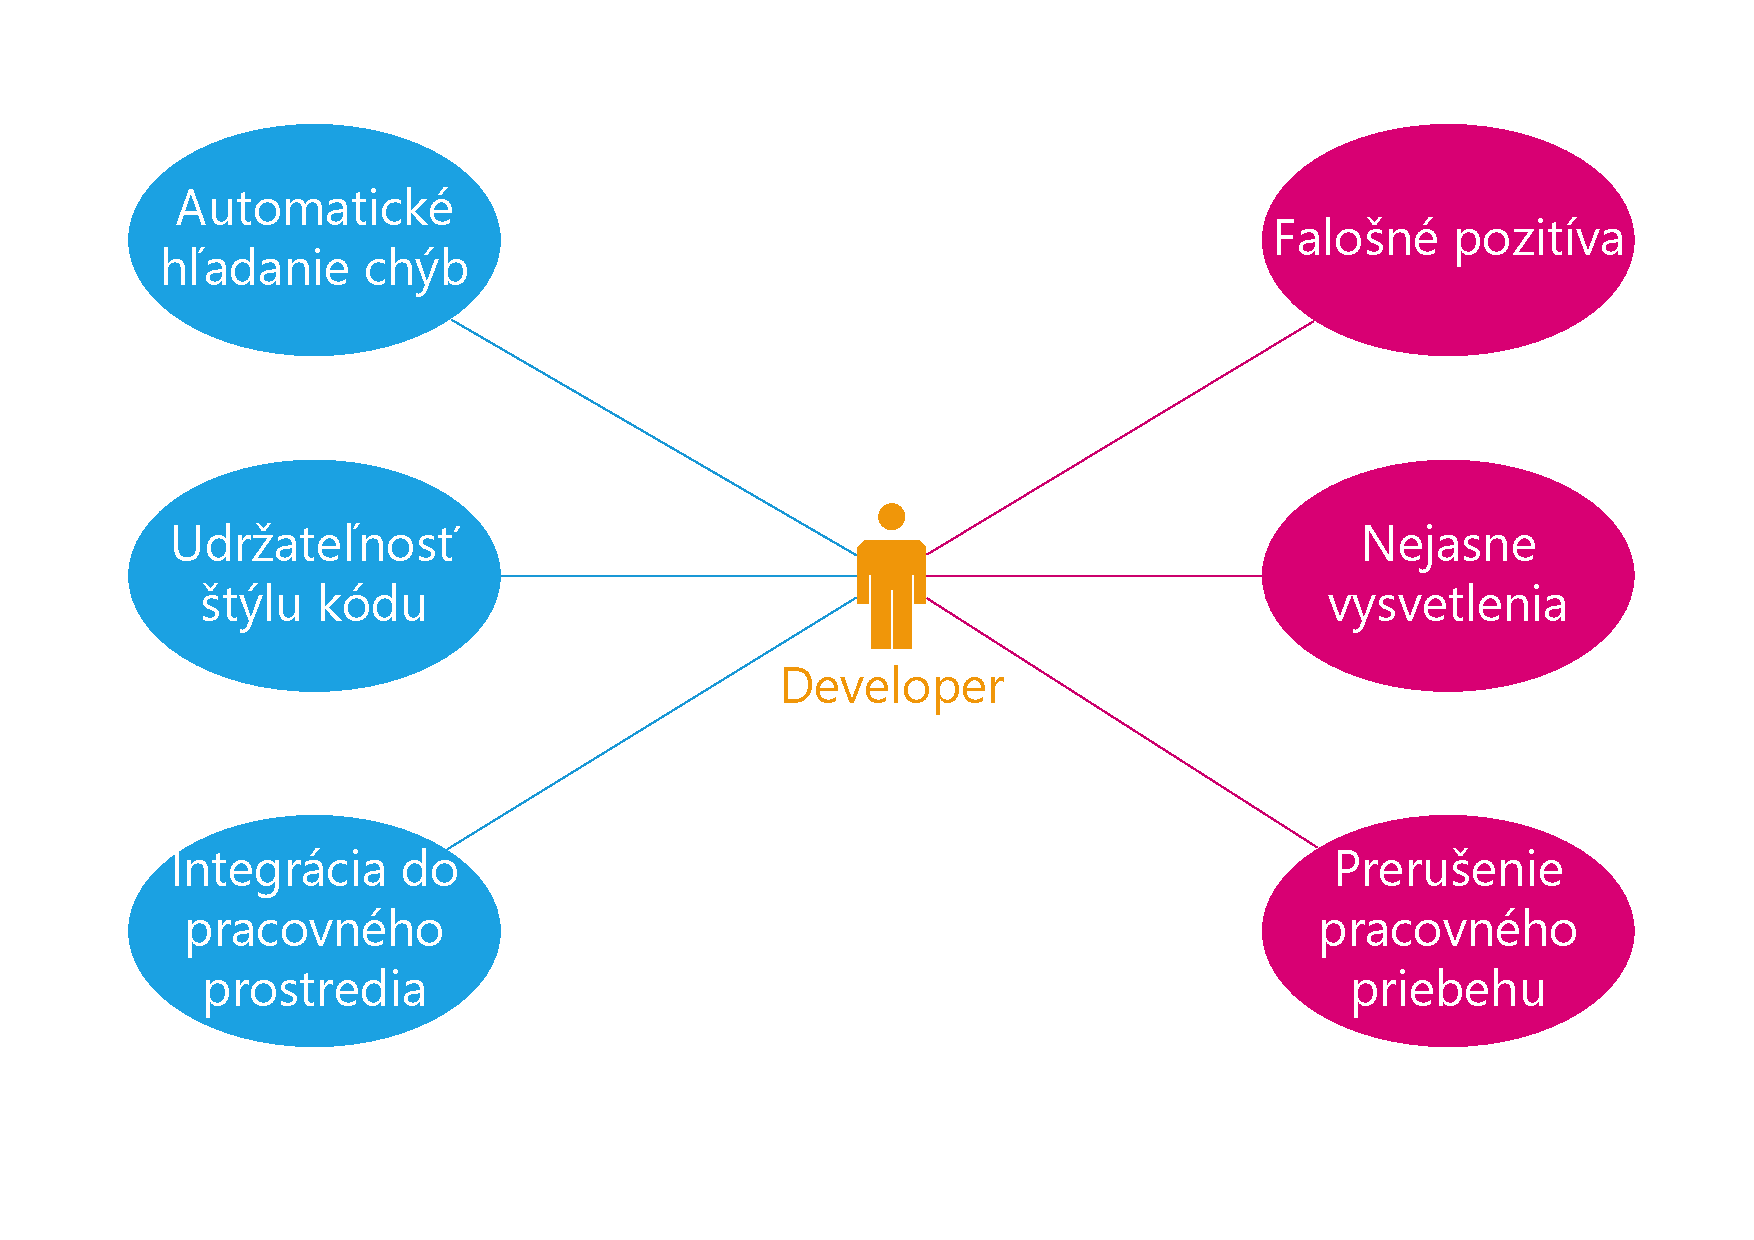
\includegraphics[scale=0.4]{pozitiva_negativa.pdf}}


% týmto sa generuje zoznam literatúry z obsahu súboru literatura.bib podľa toho, na čo sa v článku odkazujete
\bibliography{literatura}
\bibliographystyle{plain} % prípadne alpha, abbrv alebo hociktorý iný
\end{document}
